\section{Planificación}
\subsection{Gannt}
\par {}
\begin{figure}[H]
\begin{center}
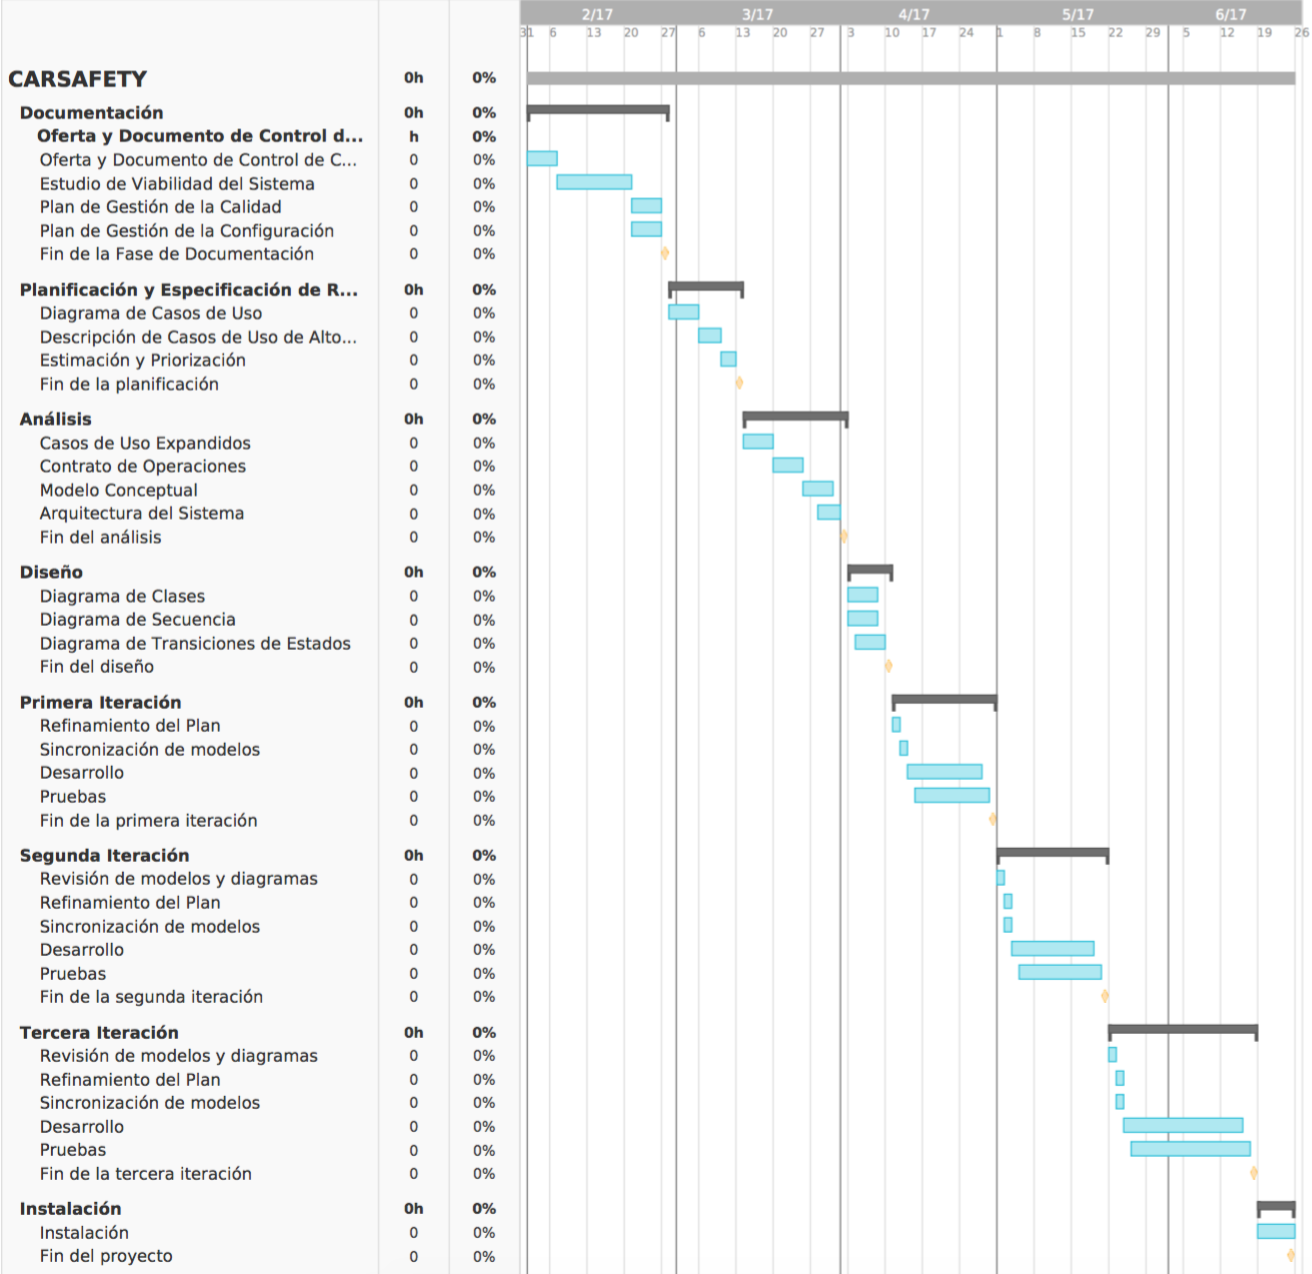
\includegraphics[width=1\textwidth]{./img/gannt.png}
\end{center}
\caption{Horas invertidas por cada miembro del equipo}
\label{tab:horasMiembro}
\end{figure}
\subsection{Método de seguimiento y control de desviaciones}
\par Un seguimiento periódico de un proyecto en el que se compruebe si se está siguiendo correctamente la planificación y que gestione las desviaciones y contratiempos lo más eficientemente posible es un punto clave e imprescindible para el éxito de un proyecto.
\begin{itemize}[-]
\item \textbf{Método de seguimiento interno}
\par para poder reducir las desviaciones, todo el equipo deberá conocer la planificación y deberá ajustarse al plan establecido. Por otro lado, el Jefe de Proyecto mantendrá reuniones quincenales con los responsables de las tareas que se encuentran en proceso, realizando un informe con el fin de informar periódicamente al cliente del estado actual del proyecto. Estas reuniones se comenzarán a mantener una vez haya concluido la planificación del proyecto, y se repetirán de forma periódica durante el ciclo de vida restante del proyecto. Para valorar el estado actual y compararlo de una forma fiable con la planificación, se utilizará el método del valor conseguido, estableciendo hitos y comparándo el progreso actual con lo planificado previamente.
\item \textbf{Método de seguimiento externo}
\par quincenalmente, el Jefe de Proyecto enviará el informe del progreso actual del proyecto al cliente. Presencialmente, se realizarán reuniones mensuales para resolver dudas importantes e informar de una forma más visual, por medio de presentaciones, del progreso del proyecto. Los participantes de estas reuniones serán: el Cliente, el Analista Jefe y el Jefe de Proyecto.
\end{itemize}
